% !TeX root = document.tex
% !TeX encoding = UTF-8 Unicode

\section{Resultados e Encerramento}

\begin{slide}{Resultados Obtidos}
  \begin{itemize}
    \item \textbf{Desempenho:} Random Forest apresentou melhor equilíbrio entre as métricas.
    \item \textbf{Comparação:} KNN perdeu desempenho com alta dimensionalidade após encoding.
    \item \textbf{Leitura geral:} baseline linear ficou competitivo, porém abaixo do melhor modelo.
  \end{itemize}

  \begin{figure}
    \centering
    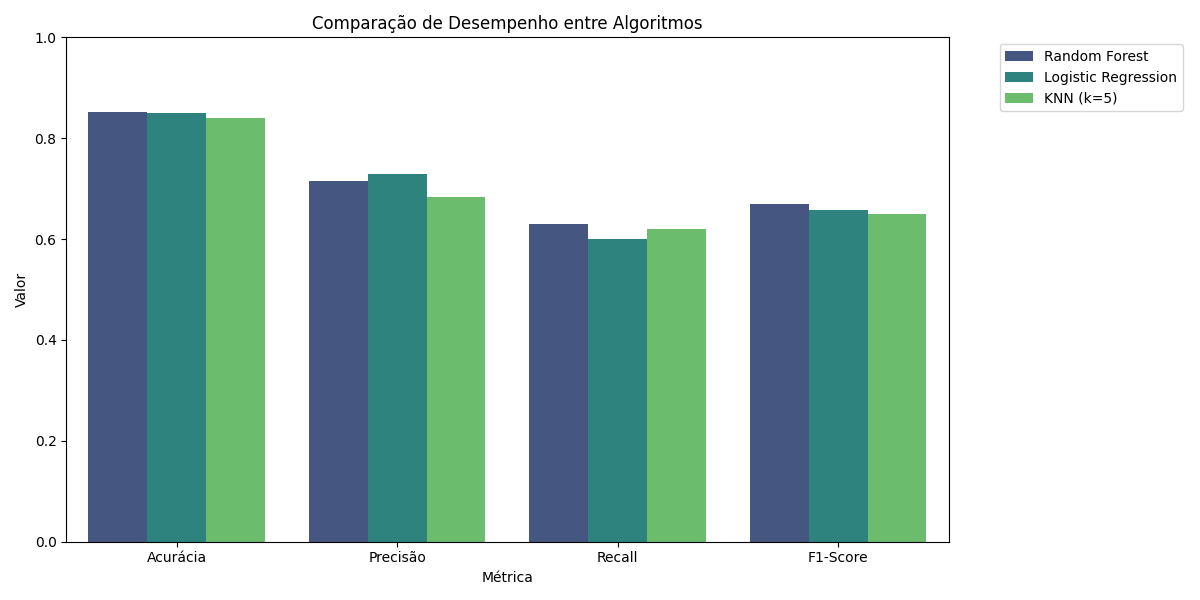
\includegraphics[width=0.78\textwidth]{../atividade_1/images/comparacao_desempenho.png}
    \caption{Comparação de desempenho entre os modelos avaliados.}
  \end{figure}
\end{slide}

\begin{slide}{Discussão e Conclusão}
  \begin{itemize}
    \item \textbf{Resumo:} pré-processamento adequado foi decisivo para a qualidade final.
    \item \textbf{Desafios:} limpeza de strings ruidosas evitou criação de classes duplicadas.
    \item \textbf{Conclusão:} a metodologia adotada permitiu análise crítica consistente dos modelos.
  \end{itemize}
\end{slide}

\begin{slide}{Referências}
  \begin{itemize}
    \item UCI Machine Learning Repository. Adult Census Income Dataset.
    \item Pedregosa et al. Scikit-learn: Machine Learning in Python.
    \item McKinney. Data Structures for Statistical Computing in Python (Pandas).
    \item Hunter. Matplotlib: A 2D Graphics Environment.
    \item Waskom. Seaborn: Statistical Data Visualization.
    \item Disciplina de Inteligência Computacional -- Prof. Dr. Alisson Marques da Silva.
  \end{itemize}
\end{slide}
